\documentclass[12pt, a4paper]{article}

% Packages and Formatting
\usepackage{../../sub/mystyle_general}
\usepackage{../../sub/mystyle_article}


\title{Lista 6 - Introdução a Análise de Dados \\
	Raspagem de dados \\
	Gabarito}
\author{Guilherme Masuko}
\date{May 2023}
%\affil{}



\definecolor{dkgreen}{rgb}{0,0.6,0}
\definecolor{gray}{rgb}{0.5,0.5,0.5}
\definecolor{mauve}{rgb}{0.58,0,0.82}

\lstset{frame=tb,
	language=R,
	aboveskip=3mm,
	belowskip=3mm,
	showstringspaces=false,
	columns=flexible,
	basicstyle={\small\ttfamily},
	numbers=none,
	numberstyle=\tiny\color{gray},
	keywordstyle=\color{blue},
	commentstyle=\color{dkgreen},
	stringstyle=\color{mauve},
	breaklines=true,
	breakatwhitespace=true,
	tabsize=3
}

\lstset{inputencoding=utf8/latin1}


\begin{document}
	
% Title Page
\clearpage
\maketitle
\thispagestyle{empty}


Vamos estudar como três variáveis macroeconomicas brasileiras se relacionam. 

\begin{itemize}
	\item Inflação
	\item Taxa de Juros
	\item Ibovespa
\end{itemize}

Para cada um desses indicadores, utilizaremos uma base de dados na forma de série temporal. 



\textbf{Questão 1}

Faça a importação dos dados. Certifique-se de manter seu diretório organizado. Exemplo:

\begin{figure}[H]
	\caption{Diretório de Exemplo}
	\centering
	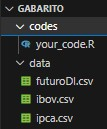
\includegraphics[scale=1]{images/directory.jpg}
\end{figure}



\lstinputlisting[language=R]{codes/your_code.R}



\begin{itemize}
	\item[\textbf{a)}] Faça a importação do arquivo \texttt{'futuroDI.csv'} em um dataframe. Utilizaremos o futuro DI\footnote{\url{https://www.bradescocorretora.com.br/SiteBradescoCorretora/Produtos/Mercados-Futuros/Produtos-Oferecidos/DI-Futuro}} como proxy da taxa de juros brasileira (Selic). Essa base de dados é composta de 22 colunas contendo dados de Junho de 2012 à Outubro de 2022. Abaixo descrevemos os dados.
	
	\begin{itemize}
		\item \texttt{X}: Data
		\item \texttt{BRPRE\_\_.BMF}: é a taxa do futuro DI onde os \_\_ são preenchidos pelo horizonte à frente referente à expectativa de taxa de juros, ex: 1M representa o futuro DI um mês à frente. Fonte: Reuters.
	\end{itemize}
	
	
	
	\textbf{Solução}
	
 	\lstinputlisting[language=R]{codes/solution1a.R}
	
	
	
	\item[\textbf{b)}] Faça a importação do arquivo \texttt{'ipca.csv'} em um dataframe. Essa base de dados é composta de 2 colunas contendo dados de Junho de 2012 à Abril de 2023. Abaixo descrevemos os dados.
	
	\begin{itemize}
		\item \texttt{X}: Data
		\item \texttt{valor}: Variação da inflação do mês anterior em relação ao mês atual.
	\end{itemize}
	
	
	\textbf{Solução}

	\lstinputlisting[language=R]{codes/solution1b.R}	
	
	
	
	\item[\textbf{c)}] Faça a importação do arquivo \texttt{'ibov.csv'} em um dataframe. Essa base de dados é composta de 2 colunas contendo dados de Junho de 2012 à Abril de 2023. Abaixo descrevemos os dados.
	
	\begin{itemize}
		\item \texttt{X}: Data
		\item \texttt{IBOV}: Pontos da bolsa brasileira Ibovespa.
	\end{itemize}
	
	
	
	\textbf{Solução}

	\lstinputlisting[language=R]{codes/solution1c.R}
	
	
	
\end{itemize}



\textbf{Questão 2}

Para cada um dos dataframes, transforme a coluna \texttt{X} em índice (nome das linhas).



\textbf{Solução}

\lstinputlisting[language=R]{codes/solution2.R}



\textbf{Questão 3}

Para cada dataframe, faça as alterações abaixo:

\begin{itemize}
	\item[\textbf{a)}] Para o dataframe \texttt{futuroDI}, mantenha somente a coluna referente ao futuro DI para um mês.
	
	
	
	\textbf{Solução}
	
	\lstinputlisting[language=R]{codes/solution3a.R}
	
	
	
	\item[\textbf{b)}] Para o dataframe \texttt{ipca}, mantenha somente a \texttt{valor}.
	
	
	
	\textbf{Solução}
	
	\lstinputlisting[language=R]{codes/solution3b.R}
	
	
	
	\item[\textbf{c)}] Para o dataframe \texttt{ibov}, mantenha somente a \texttt{IBOV}.
	
	
	
	\textbf{Solução}
	
	\lstinputlisting[language=R]{codes/solution3c.R}
	
	
	
\end{itemize}



\textbf{Questão 4}

Renomeie as colunas remanescentes para os dataframes \texttt{futuroDI}, \texttt{ipca} e \texttt{ibov}, de \texttt{BRPRE1M.BMF}, \texttt{valor} e \texttt{IBOV}, para \texttt{Futuro\_DI}, \texttt{IPCA} e \texttt{Ibovespa}.



\textbf{Solução}

\lstinputlisting[language=R]{codes/solution4.R}



\textbf{Questão 5}

Precisamos fazer manipulações no dataframe \texttt{ipca} para que cada linha tome o valor acumulado da inflação dos últimos 12 meses (assim como o Banco Central mede em \url{https://www.bcb.gov.br/}). Obtemos essa medida calculando a seguinte formula.

\begin{align*}
	\pi_{12t} &= \prod_{j=0}^{11} (1+\pi_{t-j}) - 1\\
	&= (1+\pi_t)\cdot (1+\pi_{t-1})\cdot ... \cdot (1+\pi_{t-11}) - 1
\end{align*}
onde $\pi$ é a inflação.

Para isso, siga os passos:

\begin{itemize}
	\item Crie colunas com os valores defasados. Seu dataframe deve ficar da seguinte maneira.
	
	\begin{figure}[H]
		\caption{Dataframe do IPCA}
		\centering
		\includegraphics[scale=.63]{images/ipca\_df.jpg}
	\end{figure}

	

	\textbf{Solução}
	
	\lstinputlisting[language=R]{codes/solution5a.R}
	
	
	
	\item Compute $\pi_{12t}$. Chame essa coluna de \texttt{IPCA\_Acumulado}.
	
	
	
	\textbf{Solução}
	
	\lstinputlisting[language=R]{codes/solution5b.R}
	
	
	
	\item Mantenha apenas a colunas \texttt{IPCA\_Acumulado} no dataframe \texttt{ipca}.
	
	
	\textbf{Solução}
	
	\lstinputlisting[language=R]{codes/solution5c.R}
	
	
	
\end{itemize}



\textbf{Questão 6}

\begin{itemize}
	\item[\textbf{a)}] Una os três dataframes: \texttt{futuroDI}, \texttt{ipca} e \texttt{ibov}.
	
	
	
	\textbf{Solução}
	
	\lstinputlisting[language=R]{codes/solution6a.R}
	
	
	
	\item[\textbf{b)}] Drope todas linhas que tenham \texttt{NA} em alguma das colunas.
	
	
	
	\textbf{Solução}
	
	\lstinputlisting[language=R]{codes/solution6b.R}
	
	
	
\end{itemize}

O dataframe final deve parecer como:

\begin{figure}[H]
	\caption{Dataframe Final}
	\centering
	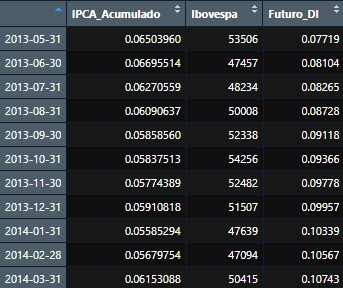
\includegraphics[scale=.63]{images/df.jpg}
\end{figure}



\textbf{Questão 7}

Calcule e interprete as correlações entre as variáveis:

\begin{itemize}
	\item \texttt{IPCA\_Acumulado} e \texttt{Futuro\_DI}.
	
	
	
	\textbf{Solução}
	
	\lstinputlisting[language=R]{codes/solution7a.R}
	
	
	
	\item \texttt{Ibovespa} e \texttt{Futuro\_DI}.
	
	
	
	\textbf{Solução}
	
	\lstinputlisting[language=R]{codes/solution7b.R}
	
	
	
\end{itemize}


	
\end{document}